\documentclass[9pt]{beamer}
\usepackage[utf8]{inputenc}
\usepackage[T1]{fontenc}
\usepackage{amsmath}
\usepackage{amsfonts}
\usepackage{amssymb}
\usepackage{graphicx}
\usetheme{CambridgeUS}

\usepackage{fontspec}
\setmainfont{Arial}
\usepackage{multimedia}
\usepackage{hyperref}
\usepackage{color}

\usepackage{xeCJK}


\title{\textbf{The Introduction of RobotSDK}}
\subtitle{A Top-down Modular Software Development Framework\\一种自顶向下的模块化软件开发框架}
\author{HMW-Alexander\\何梦文}
\logo{
\includegraphics[width=0.1\textwidth]{./logo}}
\institute[CMU]{Carnegie Mellon University\\卡内基梅隆大学}
%\date{}
%\subject{}
%\setbeamercovered{transparent}
%\setbeamertemplate{navigation symbols}{}

\begin{document}
	\maketitle
	
	\begin{frame}{报告大纲}
		\tableofcontents
	\end{frame}
	
	\section{前言:关于本报告}
	\begin{frame}{关于本报告}
		\begin{block}{报告内容}
			\begin{itemize}
				\item 介绍什么是\textcolor{red}{模块化}的软件开发理念。
				\item 介绍什么是\textcolor{red}{自顶向下}的软件开发理念。
				\item 介绍RobotSDK是如何实现自顶向下的模块化软件开发框架。
				\item 介绍RobotSDK开源开发计划。
			\end{itemize}
		\end{block}
		\pause
		\begin{block}{注意事项}
			\begin{itemize}
				\item \textcolor{red}{自顶向下的模块化软件开发理念}是本报告的关键。
				\item 而RobotSDK本身并不是本报告的重点:
				\begin{itemize}
					\item RobotSDK只是实现了自顶向下的模块化软件开发理念。但其目前还是实验室的试验品。
					\item 虽然经过多次技术升级,但是毕竟个人能力有限,所以从技术层面上是无法与成熟的软件系统开发平台(如ROS)相比的。
				\end{itemize}
				\item 报告的最终目的是希望推广自顶向下的模块化软件开发理念,并希望大家能够\textcolor{red}{参与到RobotSDK的开源开发计划},从而能够在技术和用户群方面可以和ROS相当。
			\end{itemize}
		\end{block}
	\end{frame}
	
	\section{什么是RobotSDK}
	\subsection{问题提出}
	\begin{frame}{问题提出}
		\begin{block}{当刚学会C/C++编程的时候,我们是如何完成大作业的呢?}
			\begin{itemize}
				\item<2-> 我们往往会根据题目的要求,直接写出一个浑然一体的程序。
				\item<2-> 结果往往是给一个新的大作业,就需要几乎重写一个新的程序。
				\item<3-> 这样的软件开发方式是低效率的,而且也不适合开发大的软件系统。
				\item<3-> 所以我们知道了使用\textcolor{red}{“模块化”}的方式提高软件编写效率和代码复用率。
			\end{itemize}
		\end{block}
		\begin{center}
			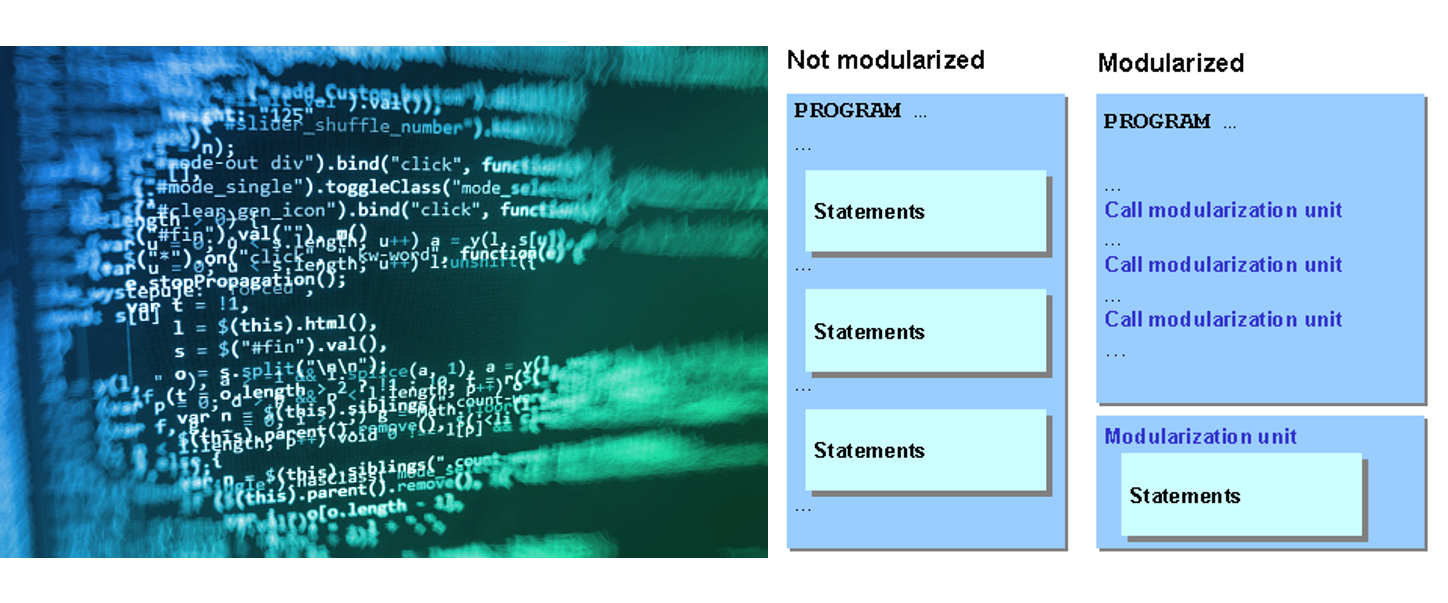
\includegraphics[width=0.8\textwidth]{./img/code}
		\end{center}
	\end{frame}
	\begin{frame}{问题提出}
		\begin{block}{当有了基本的软件开发知识和经验,我们是如何组队完成软件开发的呢?}
			\begin{itemize}
				\item<2-> 首先我们需要讨论软件的模块化设计问题,最直观的方法就是用\textcolor{red}{“图模型”}:
				\begin{itemize}
					\item 一个节点表示一个模块,定义输入输出和功能
					\item 一条有向边表示一个数据通路,定义起止节点和数据传输类型
				\end{itemize}
				\item<3-> 然后我们需要根据设计的模块与通信协议开始\textcolor{red}{分工合作开发},一般有三种方式:
				\begin{itemize}
					\item 每人编写自己对应的函数体/对象代码,最后合在一起编译成一个程序(\textcolor{red}{代码方式})
					\item 每人编写一个程序/动态库,然后用某种通信方式把所有模块组织起来(\textcolor{red}{程序方式})
					\item 上述两种方式的混合方式。
				\end{itemize}
			\end{itemize}
		\end{block}
		\begin{center}
			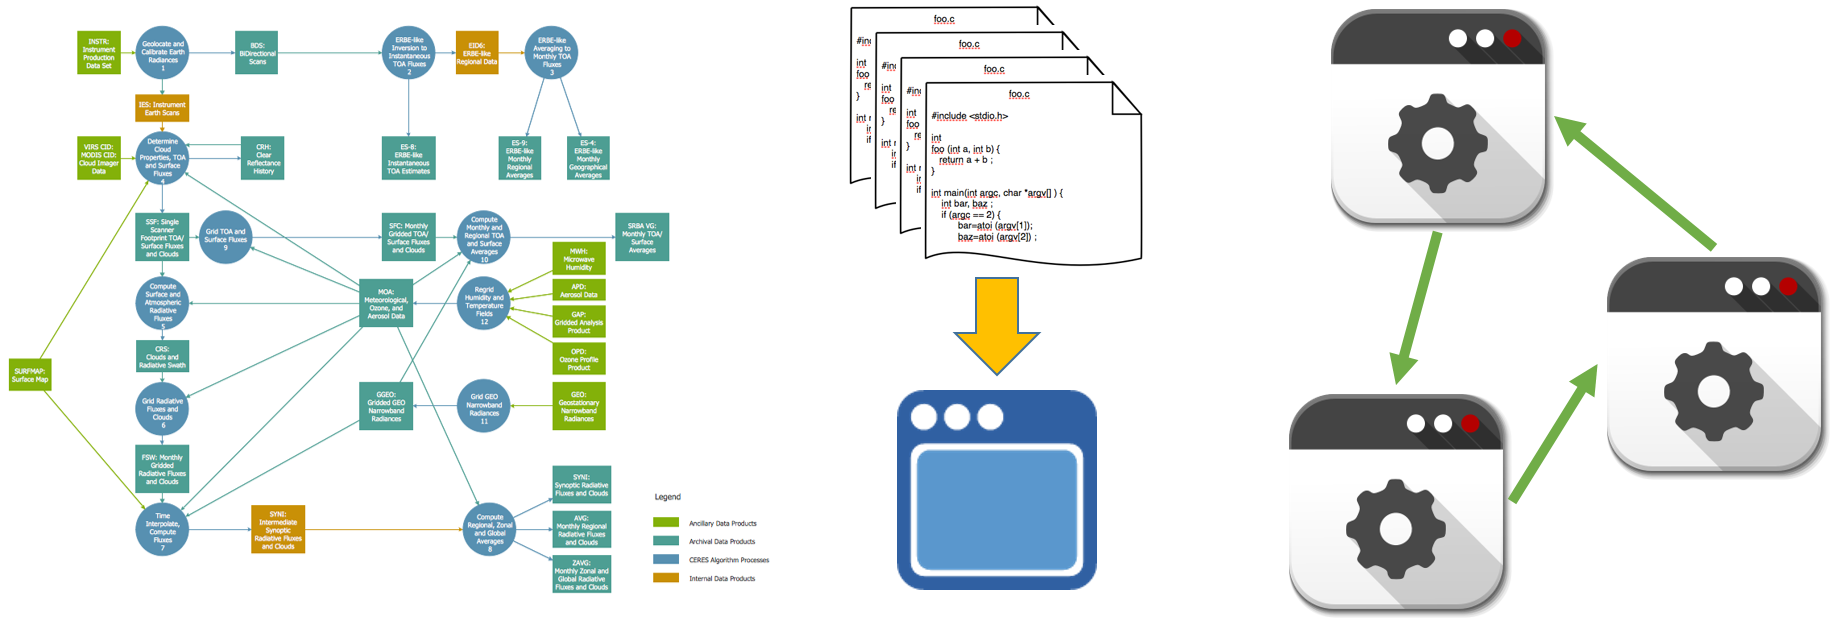
\includegraphics[width=0.8\textwidth]{./img/graph}
		\end{center}
	\end{frame}
	
	\begin{frame}{问题提出}
		\begin{block}{一、代码方式合作开发软件}
			\begin{itemize}
				\item<2-> 优点:
				\begin{itemize}
					\item 模块的功能定义非常清晰,一般直接对应算法代码本身,不需要无关辅助功能。
					\item 模块编写可以尽可能细分直到最小的函数体或对象。
					\item 数据传输一般通过参数的形式在调用函数时传递,不受数据量大小影响速度。
					\item 模块代码可以编译到静态链接库进而整合到最终软件,之后还可以被反复使用。
				\end{itemize}
				\item<3-> 缺点:
				\begin{itemize}
					\item 模块的更新一般需要重新编译整个软件,而大型软件的编译速度通常是很慢的。
					\item 模块与软件的测试一般需要等待所有相关模块编写完成并整合在一起。
					\item 软件架构(图模型的程序化)与模块高度整合,往往无法在其它工程被复用。
				\end{itemize}
			\end{itemize}
		\end{block}
		\begin{center}
			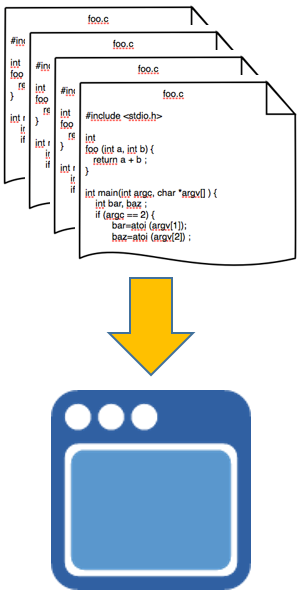
\includegraphics[width=0.2\textwidth,angle=90]{./img/way1}
		\end{center}
	\end{frame}
	\begin{frame}{问题提出}
		\begin{block}{二、程序方式合作开发软件(例如ROS)}
			\begin{itemize}
				\item<2-> 优点:
				\begin{itemize}
					\item 模块的更新无需重新编译整个软件系统。
					\item 程序化模块完成后可以自行做测试,因为其本身是独立可运行程序。
					\item 软件架构与模块是分离的,所以可以在其它工程被复用(如ROS Launch)。
					\item 程序化/动态库化模块可以被反复使用。(如ROS Package)
				\end{itemize}
				\item<3-> 缺点:
				\begin{itemize}
					\item 程序化模块还必须添加无关的辅助功能使其成为可运行程序并能与外界进行通讯。
					\item 模块编写可以尽可能细分,但为了开发效率,一般是将相关功能集整合到一个模块中。
					\item 基于网路的数据实体传输,速度会受数据量大小影响。(ROS是基于网络的指针传输)
				\end{itemize}
			\end{itemize}
		\end{block}
		\begin{center}
			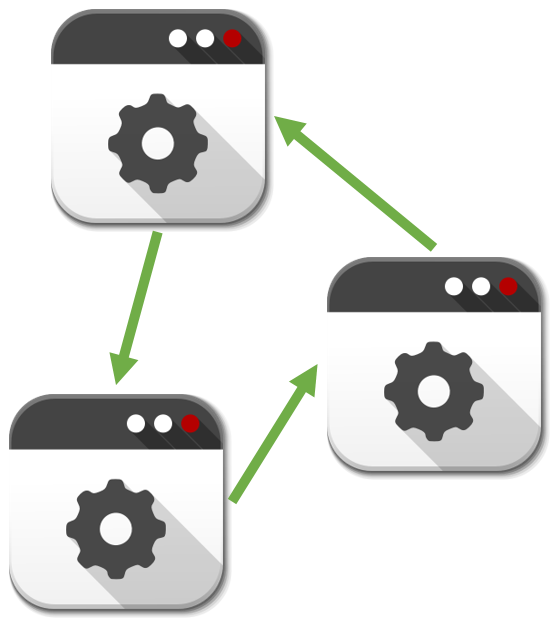
\includegraphics[width=0.2\textwidth]{./img/way2}
		\end{center}
	\end{frame}
	
	\begin{frame}{问题提出}
		\begin{block}<1->{两种方式的共有缺点}
			\begin{itemize}
				\item 软件架构只针对于特定功能的模块集合,不能泛化到类似图模型的实现。
				\item 这里涉及到\textcolor{red}{自顶(高层抽象)向下(底层实现)的软件开发理念},我们先讨论“泛化”概念。
			\end{itemize}
		\end{block}
		\begin{block}<2->{概念解释:软件架构的泛化}
			\begin{itemize}
				\item 软件架构:即程序化(实例化)的图模型,其将各个功能模块实体组织在一起发挥软件的功能。
				\item 泛化:我们通过下面一个简单例子来解释这个概念。
			\end{itemize}
		\end{block}
	\end{frame}
	\begin{frame}{问题提出}
		\begin{block}{机器人数据采集可视化存储软件系统开发实例}
			\begin{itemize}
				\item<1-> 现在有一个机器人装有Camera、LiDAR、Encoder/IMU等传感器。
				\item<2-> 我们一般会设计出如下图模型:
			\end{itemize}
		\end{block}
		\begin{center}
			\includegraphics[width=0.6\textwidth]<2->{./img/lowlevel}
		\end{center}
	\end{frame}
	\begin{frame}{问题提出}
		\begin{block}{机器人数据采集可视化存储软件系统开发实例}
			\begin{itemize}
				\item<1-> 按照上述图模型,我们需要编写三个\textcolor{red}{功能不同}的软件架构,对应各传感器。
				\item<2-> 有经验的人会用面向对象的方式高效的编写出上述三个软件架构(\textcolor{red}{代码层抽象})。
				\item<2-> 这很棒,因为你已经看出来了这三个软件架构具有相似的\textcolor{red}{“抽象图模型”}。
				\item<3-> 当来了新传感器,仍需要再编写相似结构的软件架构。(这个简单例子不是大问题)
			\end{itemize}
		\end{block}
		\begin{center}
			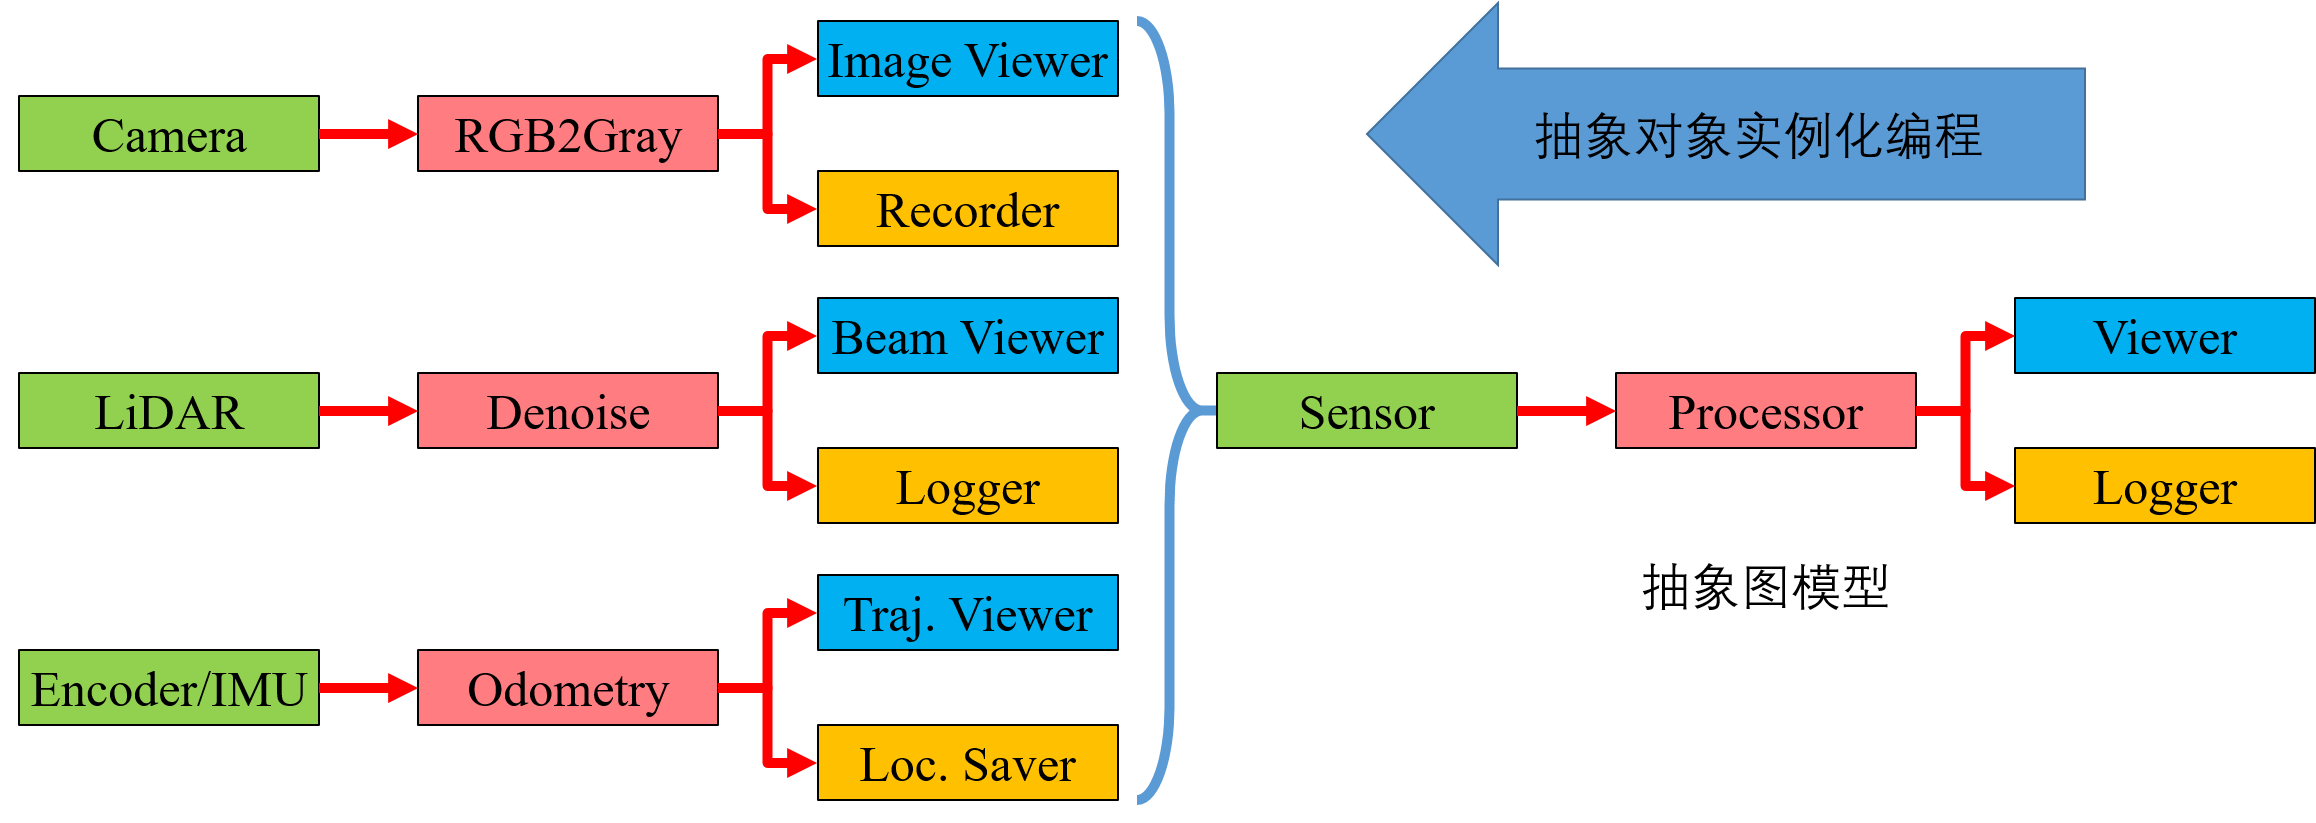
\includegraphics[width=\textwidth]{./img/highlevel}
		\end{center}
	\end{frame}
	\begin{frame}{问题提出}
		\begin{block}{机器人数据采集可视化存储软件系统开发实例}
			\begin{itemize}
				\item<1-> 实际开发中往往能发现很多软件是基于相似但很复杂的\textcolor{red}{“抽象图模型”}。
				\item<2-> 这时候,\textcolor{red}{代码层抽象}只能方便我们设计软件,但无法\textcolor{red}{减少重复编程}。
				\item<3-> 能否对于某个图模型实现软件架构后,该软件架构能够\textcolor{red}{泛化}应用到相似图模型呢?
				\item<4-> 答案是可以,即通过\textcolor{red}{程序层抽象}实现\textcolor{red}{抽象图模型}的\textcolor{red}{抽象软件架构}。
			\end{itemize}
		\end{block}
		\begin{center}
			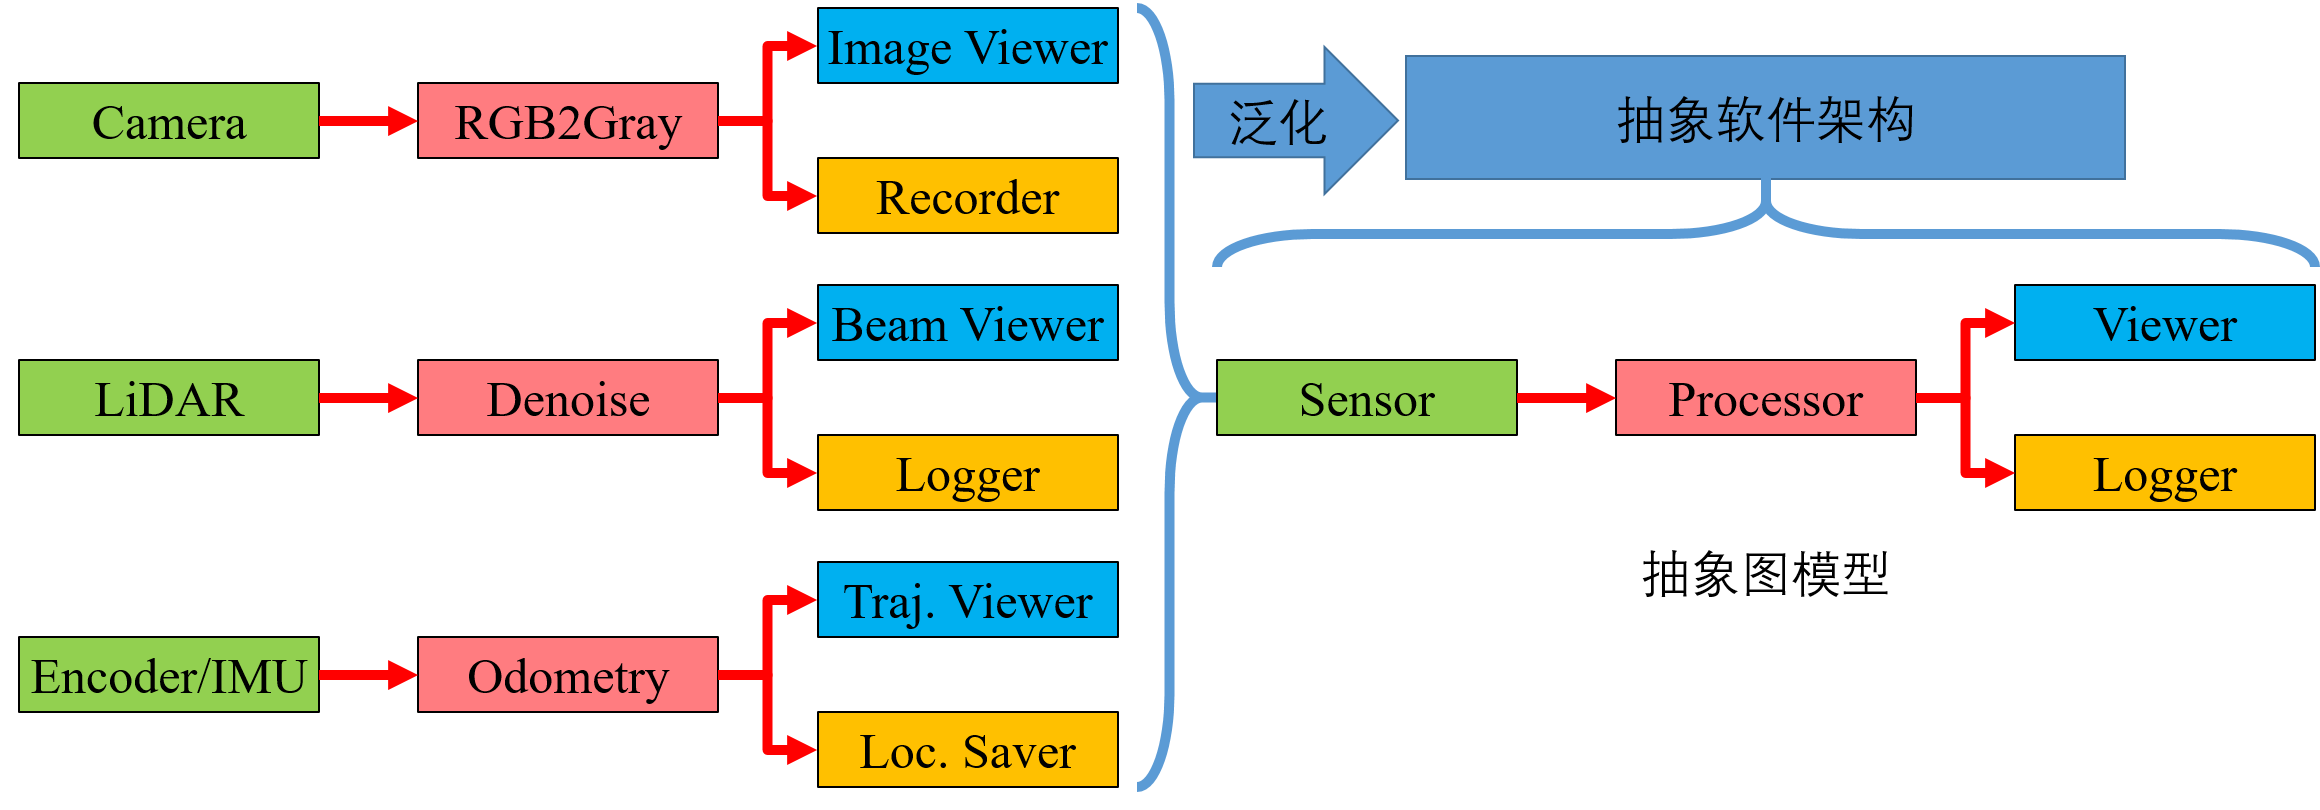
\includegraphics[width=\textwidth]{./img/highlevel1}
		\end{center}
	\end{frame}
	
	\subsection{问题总结,目标与要求}
	\begin{frame}{问题总结,目标与要求}
		\begin{block}<1->{问题总结}
			\begin{itemize}
				\item \textcolor{red}{模块化设计}是目前通用的软件设计方法,一般基于\textcolor{red}{图模型}设计。
				\item \textcolor{red}{模块化开发}是高效的分工合作软件开发方式,两种开发方式各有自己的优缺点。
				\item \textcolor{red}{软件架构的泛化}能够减少不必要的对相似图模型的编程。
			\end{itemize}
		\end{block}
		\begin{block}<2->{目标与要求}
			开发一种高效的软件开发框架:
			\begin{itemize}
				\item<3-> 提供基于图模型的模块化软件设计,并支持抽象图模型。
				\item<4-> 使其具有两种模块化开发方式的优点:
				\begin{itemize}
					\item 模块直接对应算法代码本身,不需要无关辅助功能。
					\item 模块可以高效的细分到最小函数体或对象。
					\item 模块的更新不需要重新编译整个系统。
					\item 模块间数据传输不受数据量大小影响速度。
					\item 模块可以被不同工程反复使用。
					\item 软件架构与模块分离,可以被其它工程复用。			
				\end{itemize}
				\item<5-> 利用基于抽象图模型的抽象软件架构编程实现软件架构的泛化。
			\end{itemize}
		\end{block}
	\end{frame}
	
	\subsection{关于RobotSDK}
	\subsubsection{自顶向下的模块化开发理念}
	\begin{frame}{关于RobotSDK}
		\begin{block}{自顶向下的模块化开发理念与简单说明}
			\begin{itemize}
				\item 模块化:
				\begin{itemize}
					\item 模块化开发理念无需赘言。
					\item RobotSDK通过\textcolor{red}{预制代码模板}直接封装算法代码到\textcolor{red}{动态库}实现模块化开发。
					\item 动态库模块通过\textcolor{red}{显示链接}可以自由嵌入\textcolor{red}{抽象软件架构}(RobotSDK称为高层程序)。
					\item 这种模块化开发方式满足了上述的目标与要求。
				\end{itemize}
			\end{itemize}
		\end{block}
		\begin{center}
			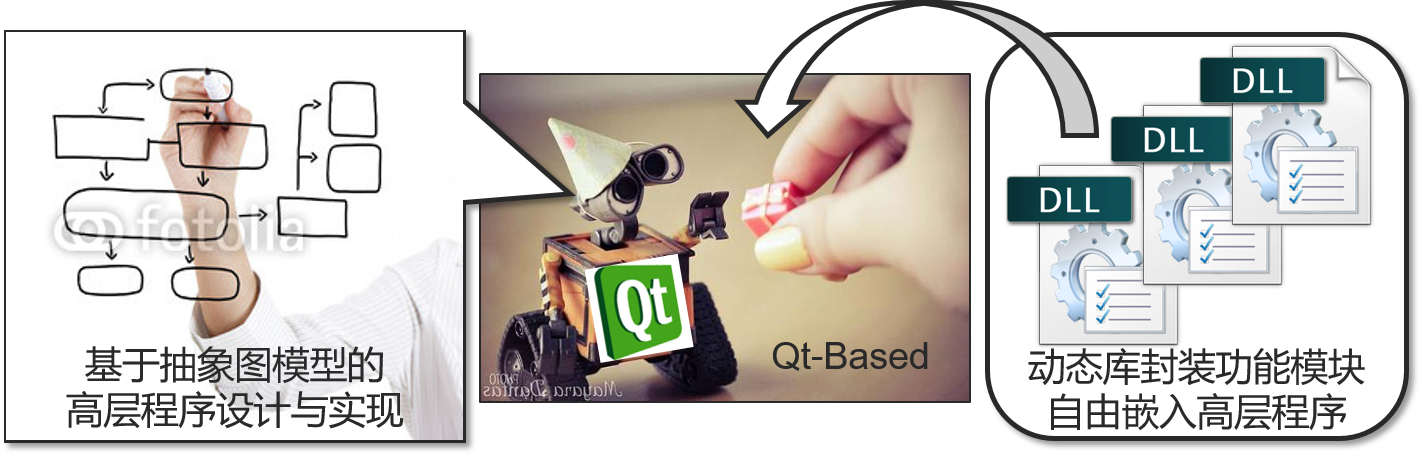
\includegraphics[width=\textwidth]{./img/idea}
		\end{center}
	\end{frame}
	\begin{frame}{关于RobotSDK}
		\begin{block}{自顶向下的模块化开发理念与简单说明}
			\begin{itemize}
				\item 自顶向下:
				\begin{itemize}
					\item<2-> 首先是一种从高层到底层的软件开发流程。
					\begin{itemize}
						\item 【高层】高层图模型的设计与高层程序的编写,只关注图模型的实现,不具有具体功能。
						\item 【底层】底层模块开发,只关注模块算法本身的编写和封装,不用考虑高层设计架构。
					\end{itemize}
					\item<3-> 其次是一种从抽象到具体的软件开发流程。
					\begin{itemize}
						\item 【抽象】抽象的高层图模型与对应的抽象软件架构实现,只关注图模型的结构实现,不具有功能。
						\item 【具体】泛化的抽象软件架构在嵌入具体的底层功能模块后,拥有了对应具体图模型的软件功能。
					\end{itemize}
				\end{itemize}
			\end{itemize}
		\end{block}
		\begin{center}
			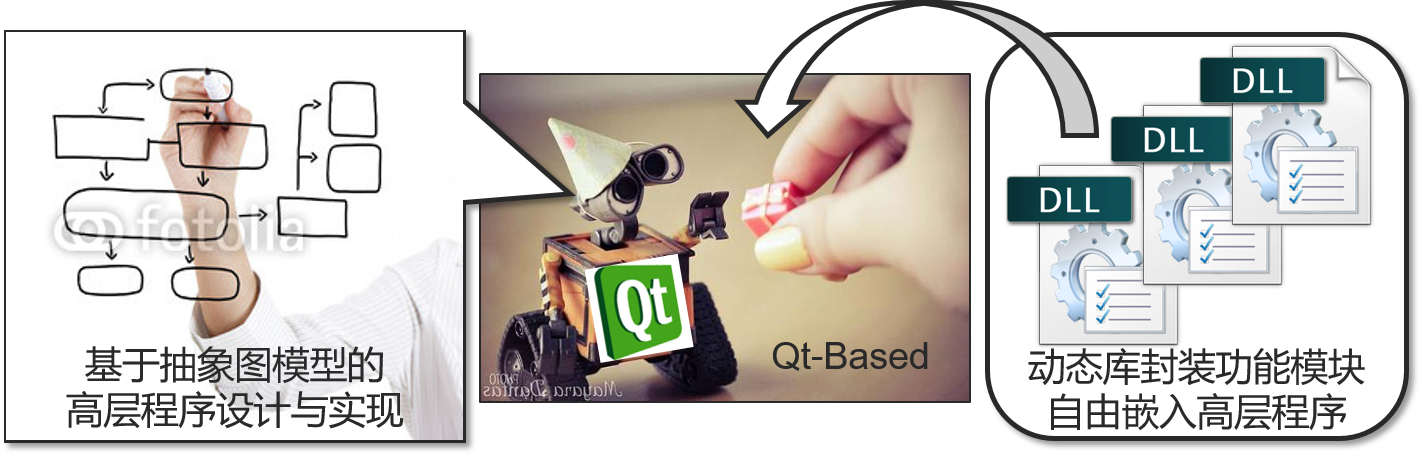
\includegraphics[width=\textwidth]{./img/idea}
		\end{center}
	\end{frame}	
	\begin{frame}[allowframebreaks]{关于RobotSDK---自顶向下的模块化开发理念实例}
		\begin{center}
			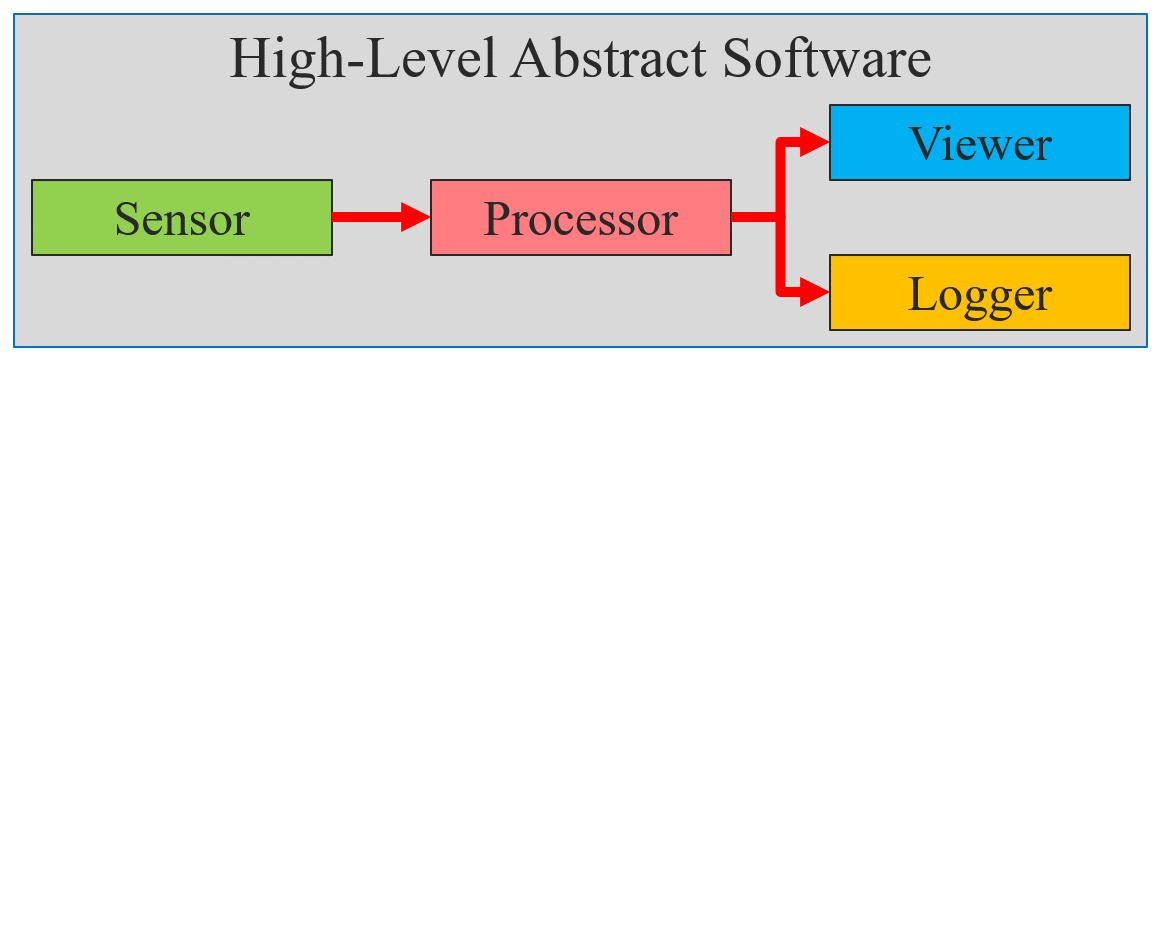
\includegraphics[width=0.7\textwidth]{./img/ex1-1}
		\end{center}
		\begin{center}
			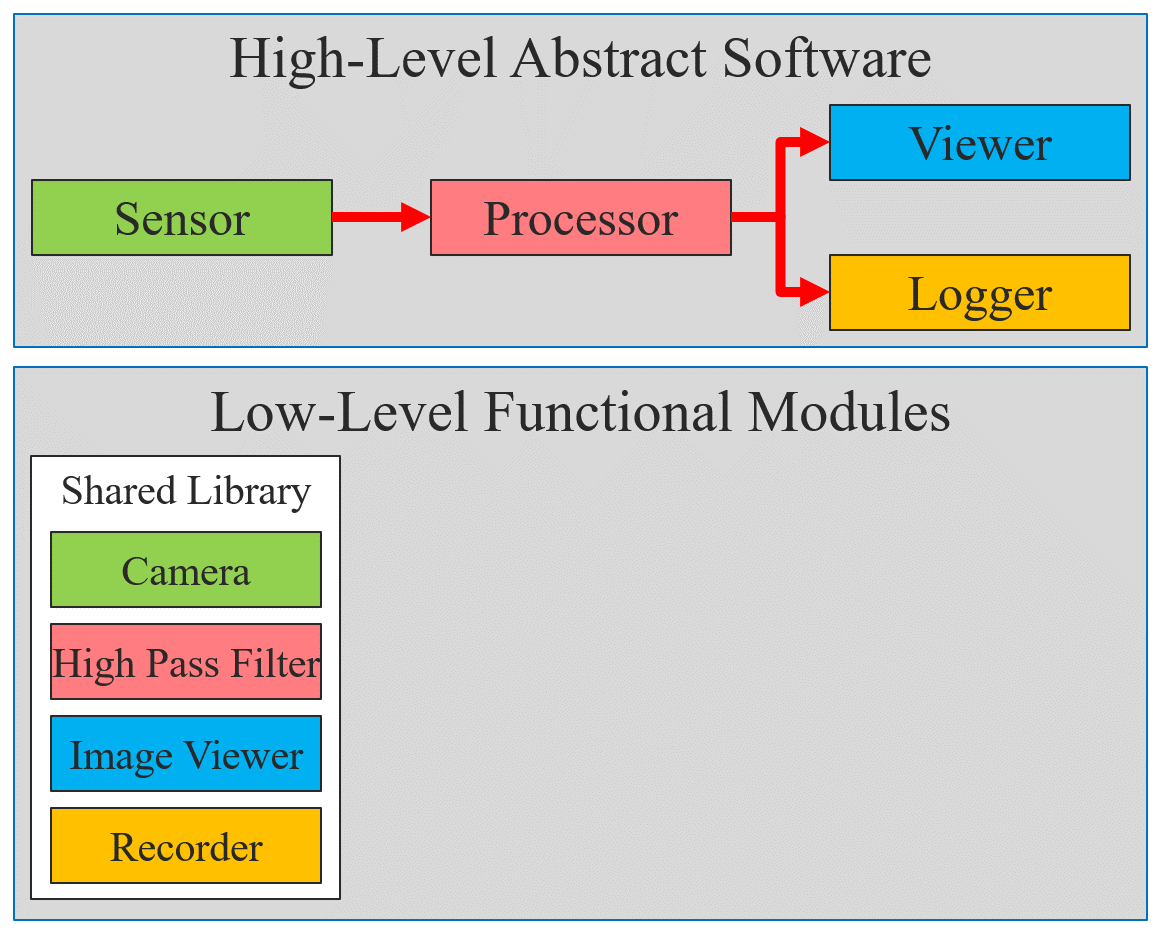
\includegraphics[width=0.7\textwidth]{./img/ex1-2}
		\end{center}
		\begin{center}
			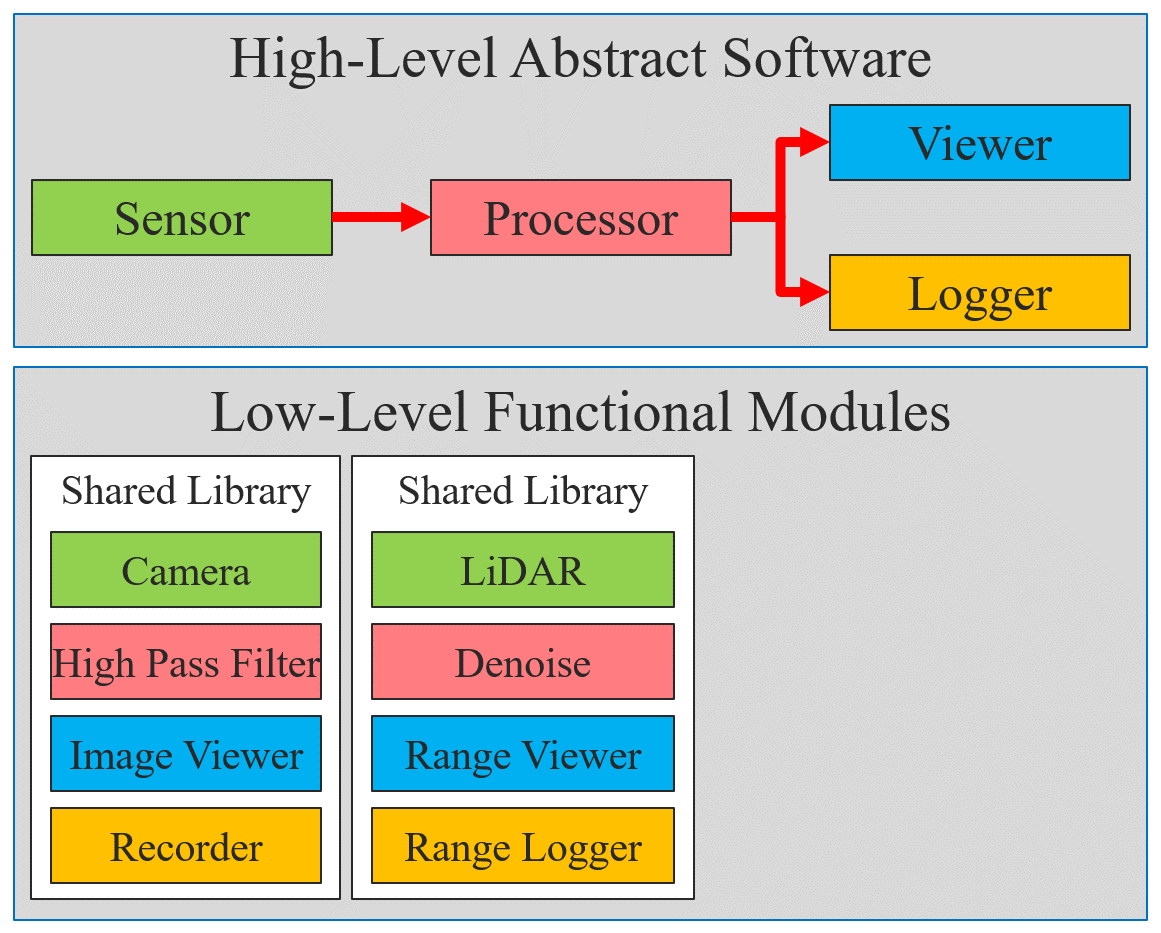
\includegraphics[width=0.7\textwidth]{./img/ex1-3}
		\end{center}
		\begin{center}
			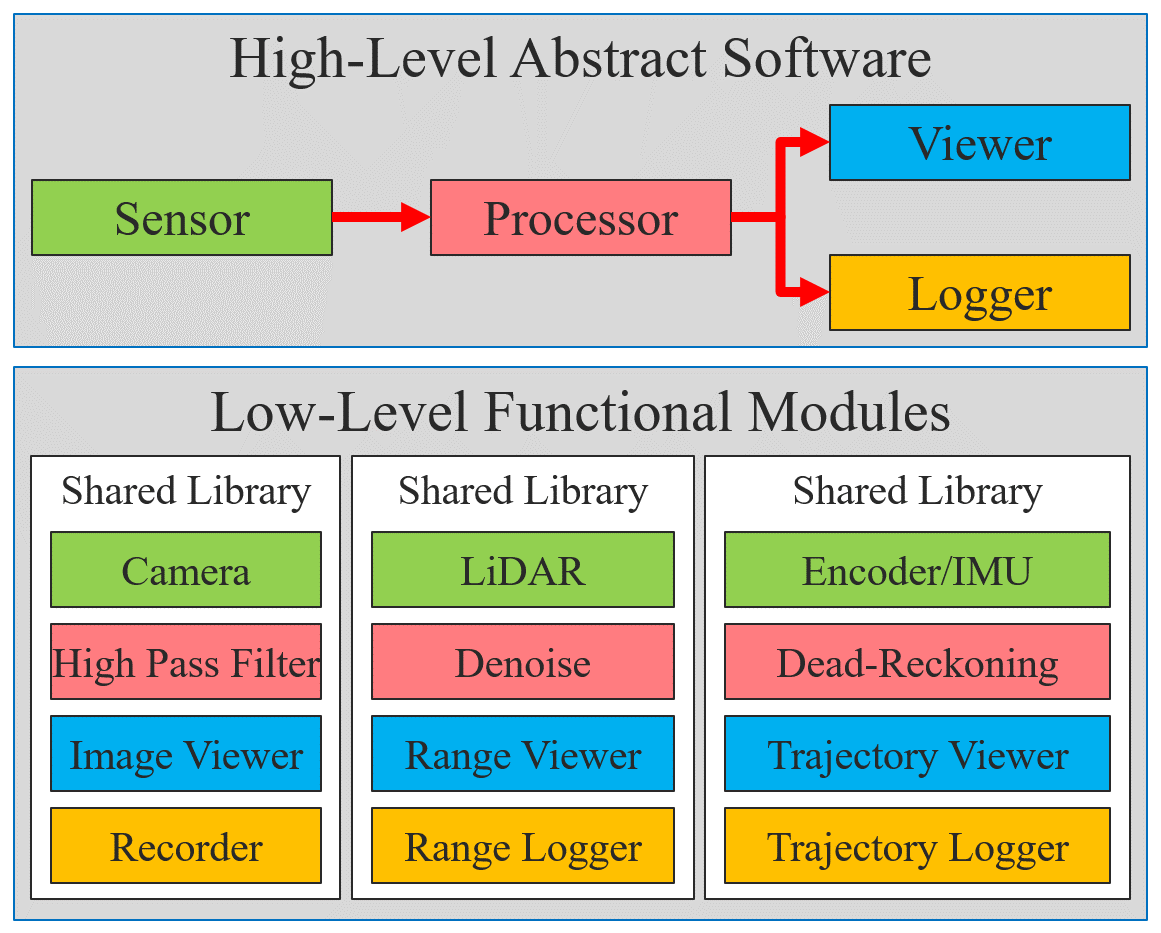
\includegraphics[width=0.7\textwidth]{./img/ex1-4}
		\end{center}
	\end{frame}
	
	\subsubsection{基本概念}
	\begin{frame}{关于RobotSDK---基本概念}
		\begin{block}{高层图模型与高层程序}
			\begin{itemize}
				\item<2-> 节点:功能模块的嵌入槽,同时定义了输入与输出端口。
				\item<3-> 有向边:通用数据指针的通讯连接。所有不同类型的数据都存放在统一的数据池中,通信只传递指针,所以通信速度不会受到数据量影响。
				\item<4-> 高层程序:只实现抽象图模型,但不具有任何实际功能。当嵌入封装了功能模块的动态库后,才具有实际功能。另外可以只插入部分功能模块,从而实现其子图的功能,可以用来做子系统测试。
				\item<5-> Robot-X:在最新的4.0版本,由于实现了脚本化高层程序,所以无需再编程实现,而是直接画图后解析即可得到高层抽象软件。Robot-X就是抽象图模型的解析器,解析完后就成为了对应该图模型的高层程序。另外,Robot-X可以同时解析多个抽象图模型,并进行图合并操作(相同节点会被合并),从而实现将简单子系统融合成复杂系统的功能。
			\end{itemize}
		\end{block}
	\end{frame}
	\begin{frame}{关于RobotSDK---基本概念}
		\begin{block}{底层功能模块}
			\begin{itemize}
				\item<2-> 预制代码模板:由RobotSDK根据图模型中的节点自动生成,其定义了功能模块与抽象节点的通信接口(底层模块开发者无需关注和了解)。底层模块开发者只需要将自己的算法代码填入算法封装区,并设计由模块“main”函数调用即可。
				\item<3-> 动态库:通过模板代码将功能模块的实现算法封装入动态库,从而通过显示链接(explicit link)的方式将功能模块嵌入高层抽象软件的节点。一个动态库可以封装任意多的功能模块,一个动态库可以被任意多的高层抽象软件使用。注意:链接了的动态库如果被更新,更新内容只会在高层抽象软件重启后才起作用,这是目前还没有解决的热插拔问题。
				\item<4-> 多线程管理与数据流驱动:Robot-X自动为每个嵌入的功能模块提供单独的线程,无需底层开发者额外设计。同时基于图模型的软件架构本身存在“源”和“漏”两种节点,所以处于不同线程的模块是通过从“源”到“漏”的数据流驱动进行同步的,这一点也无需底层开发者做额外设计。
			\end{itemize}
		\end{block}
	\end{frame}
	
	\subsubsection{基本架构}
	\begin{frame}[allowframebreaks]{什么是RobotSDK---基本架构}
		\begin{center}
			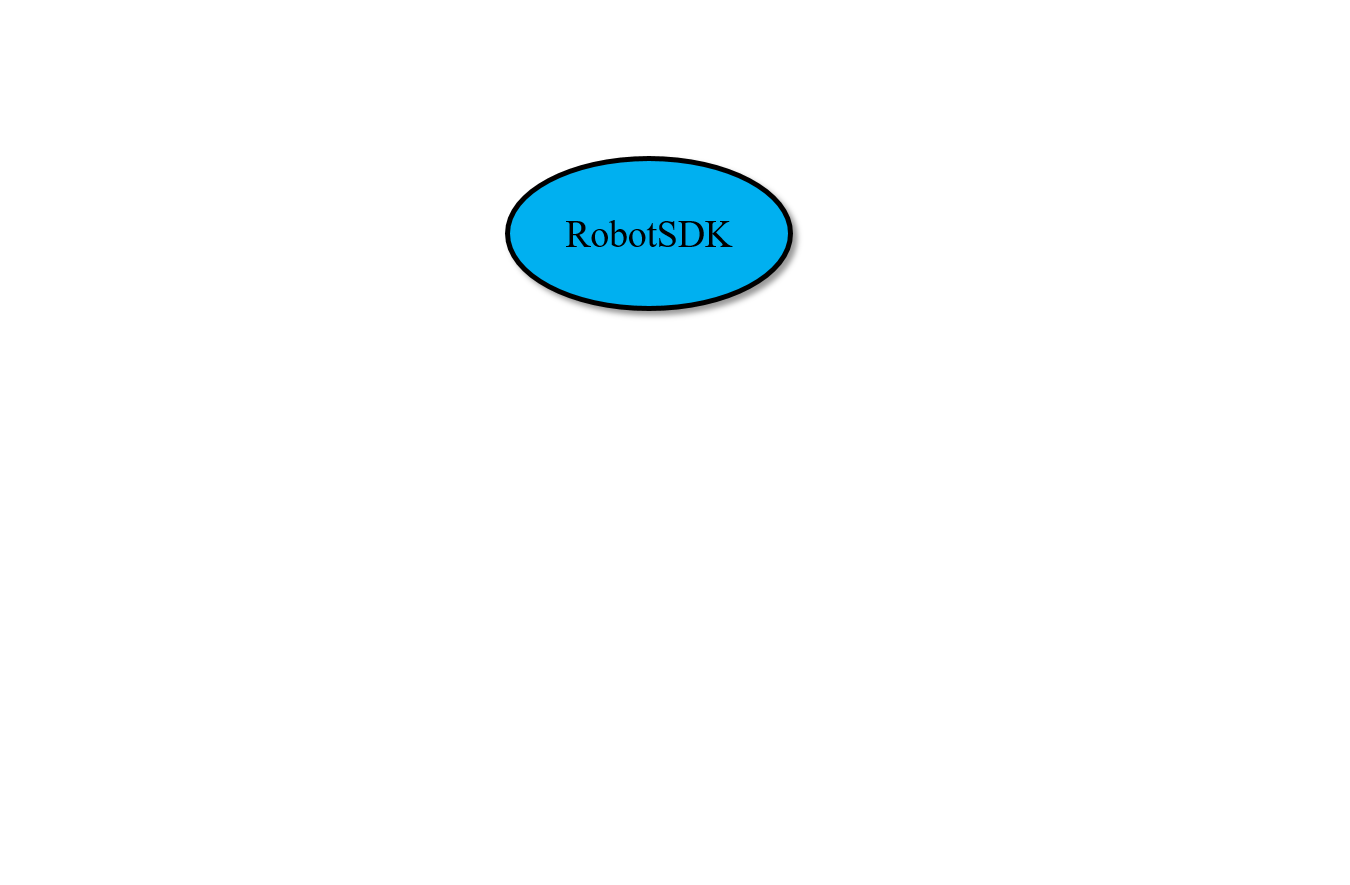
\includegraphics[width=0.9\textwidth]{./img/frame1}
		\end{center}
		\begin{center}
			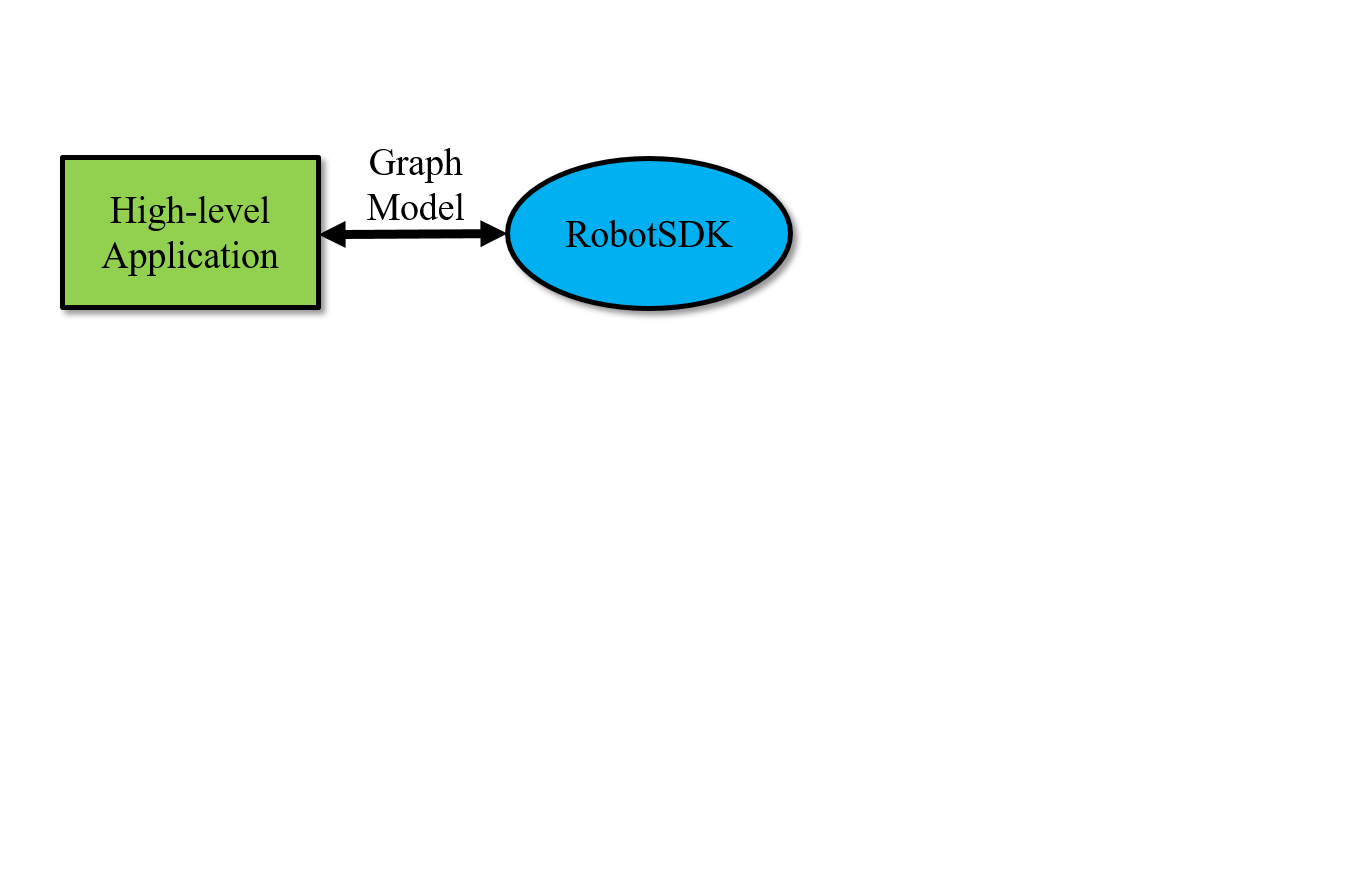
\includegraphics[width=0.9\textwidth]{./img/frame2}
		\end{center}
		\begin{center}
			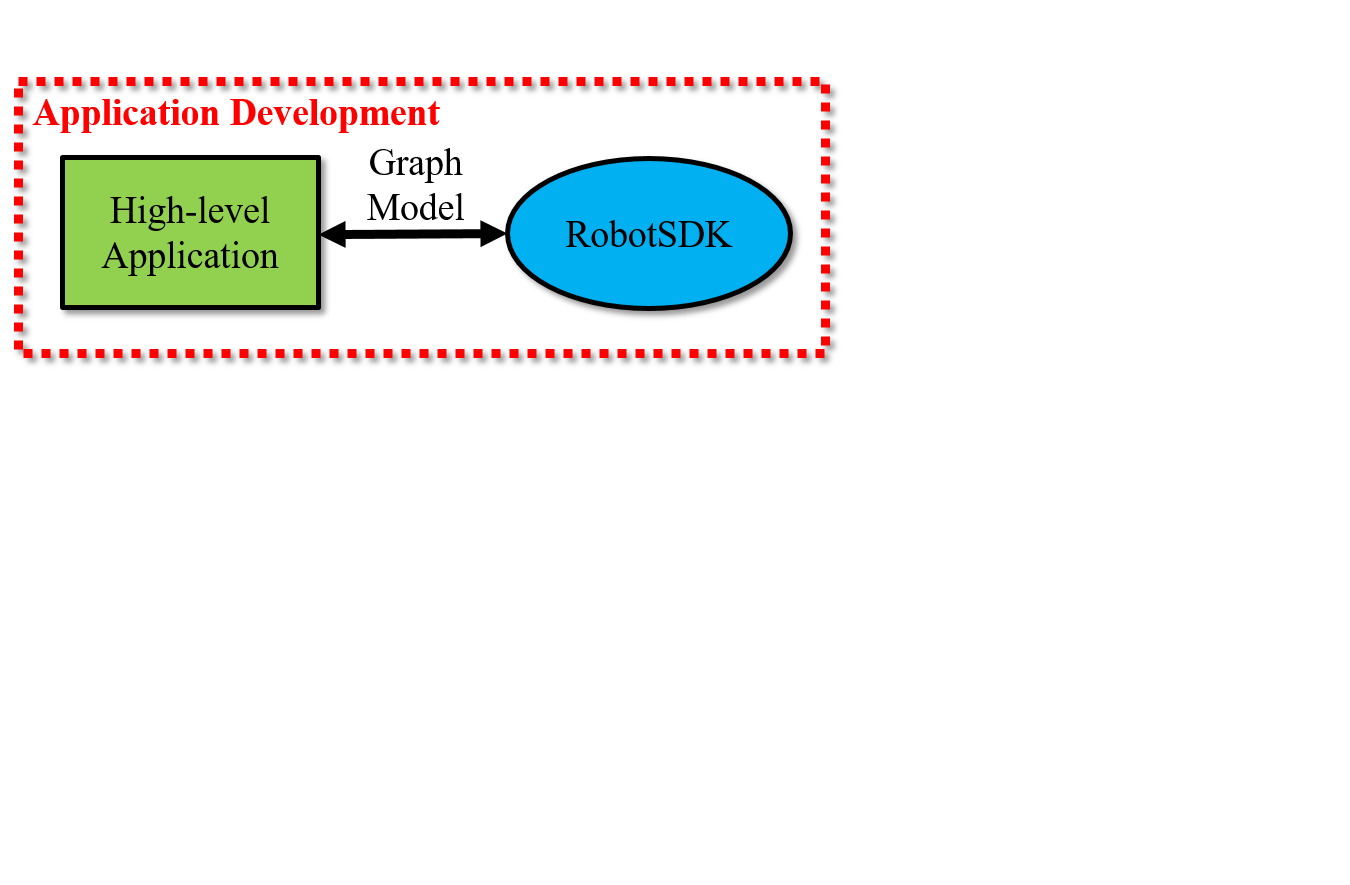
\includegraphics[width=0.9\textwidth]{./img/frame3}
		\end{center}
		\begin{center}
			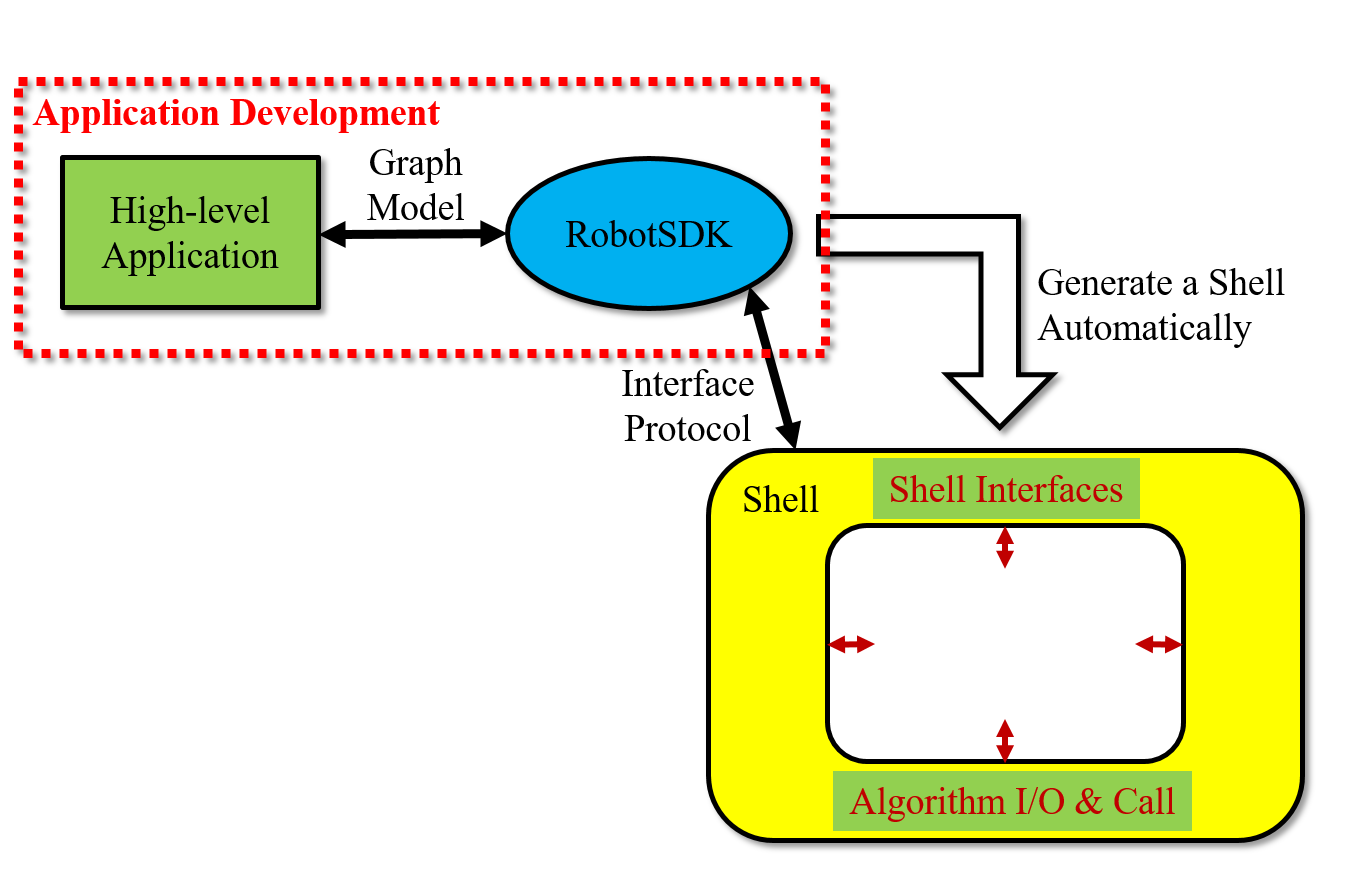
\includegraphics[width=0.9\textwidth]{./img/frame5}
		\end{center}
		\begin{center}
			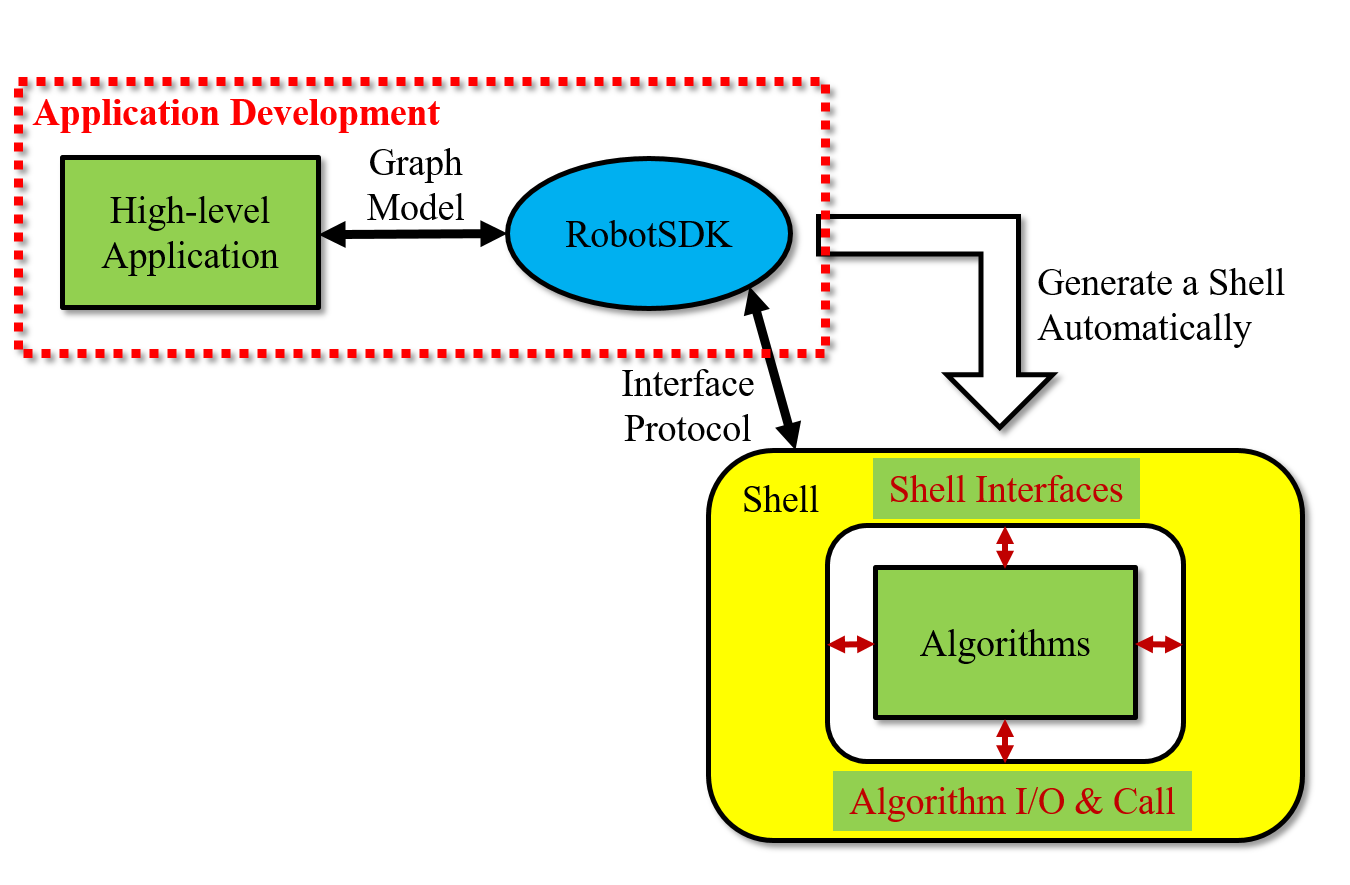
\includegraphics[width=0.9\textwidth]{./img/frame6}
		\end{center}
		\begin{center}
			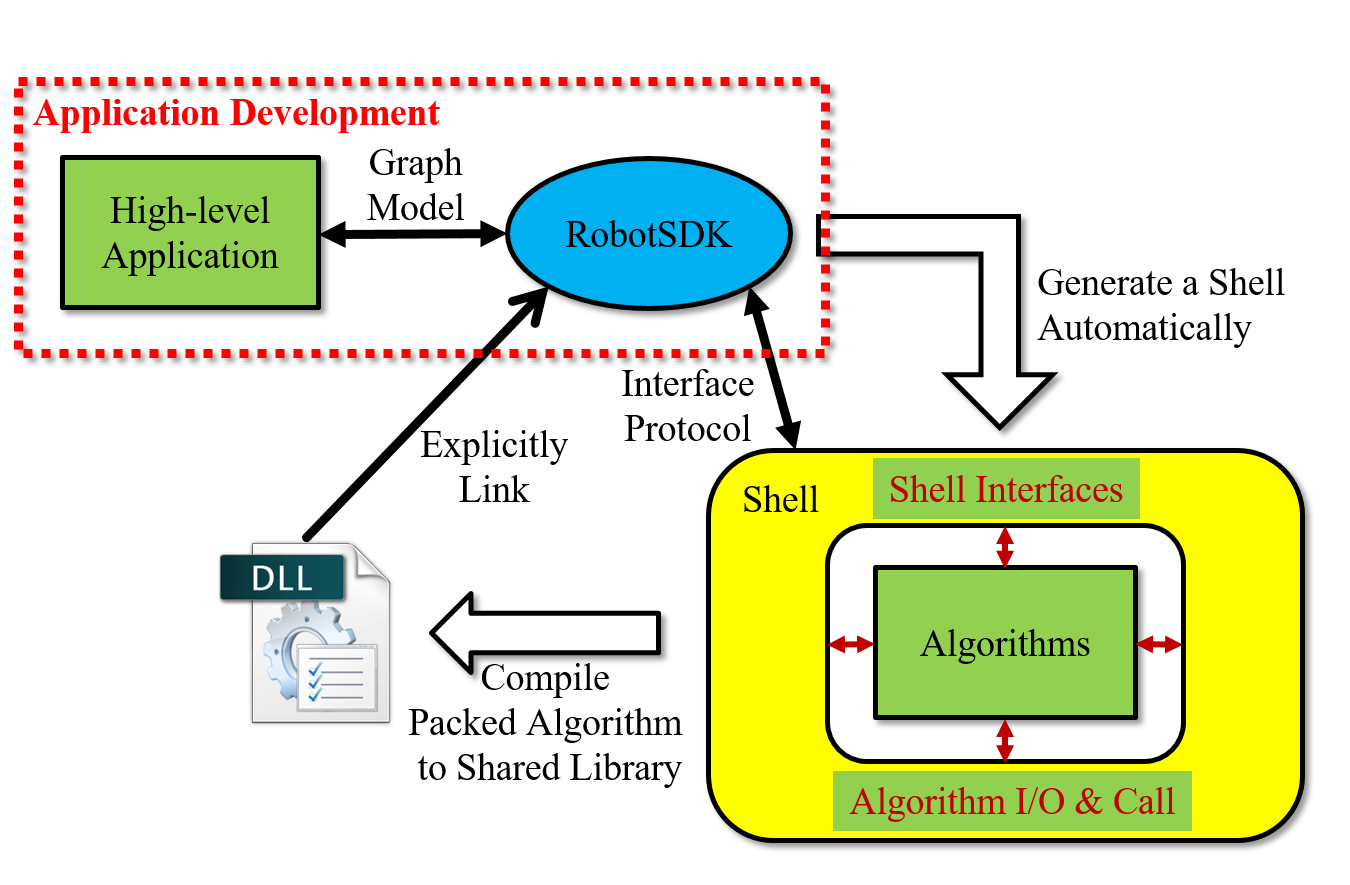
\includegraphics[width=0.9\textwidth]{./img/frame7}
		\end{center}
		\begin{center}
			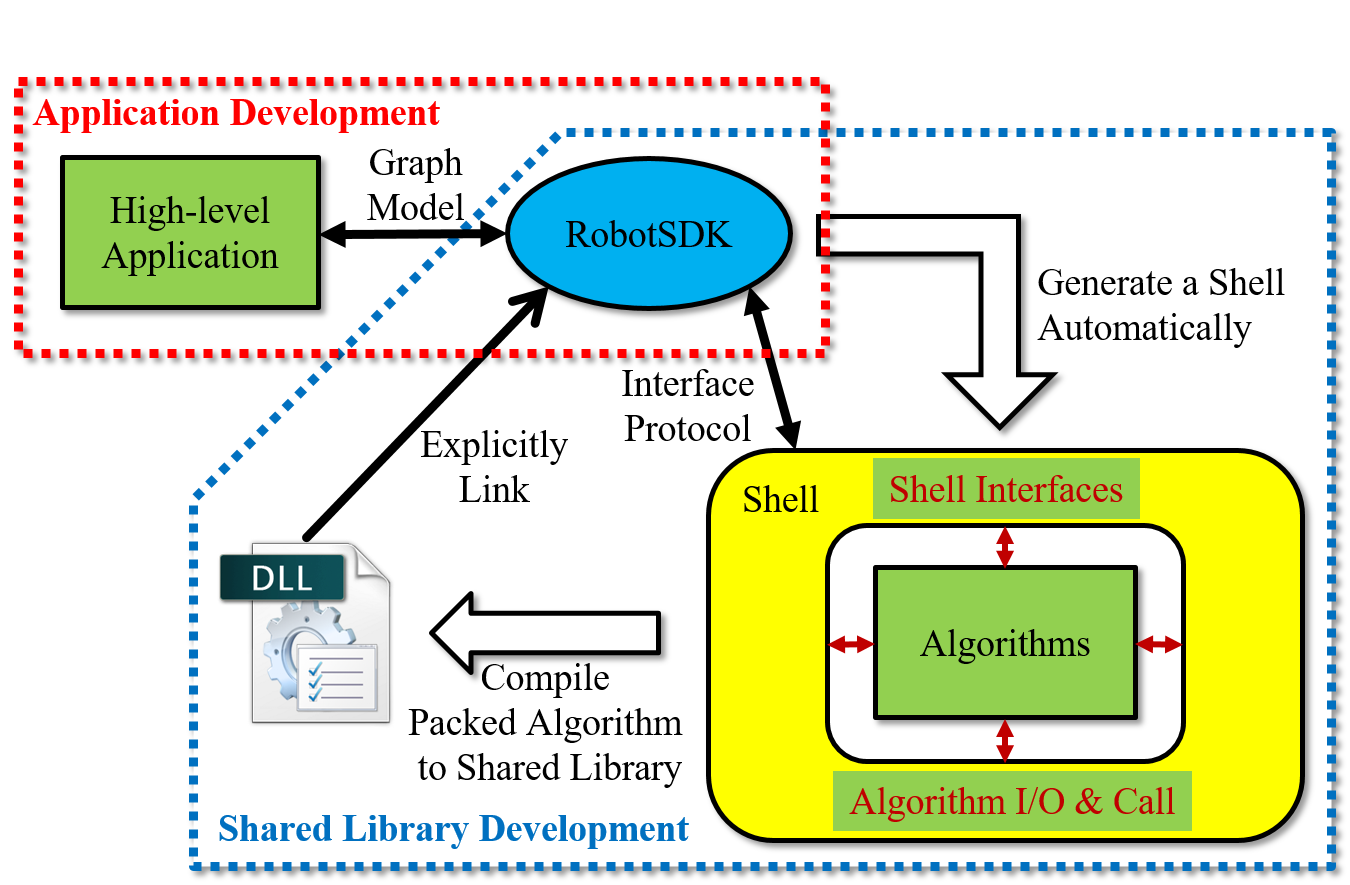
\includegraphics[width=0.9\textwidth]{./img/frame8}
		\end{center}
		\begin{center}
			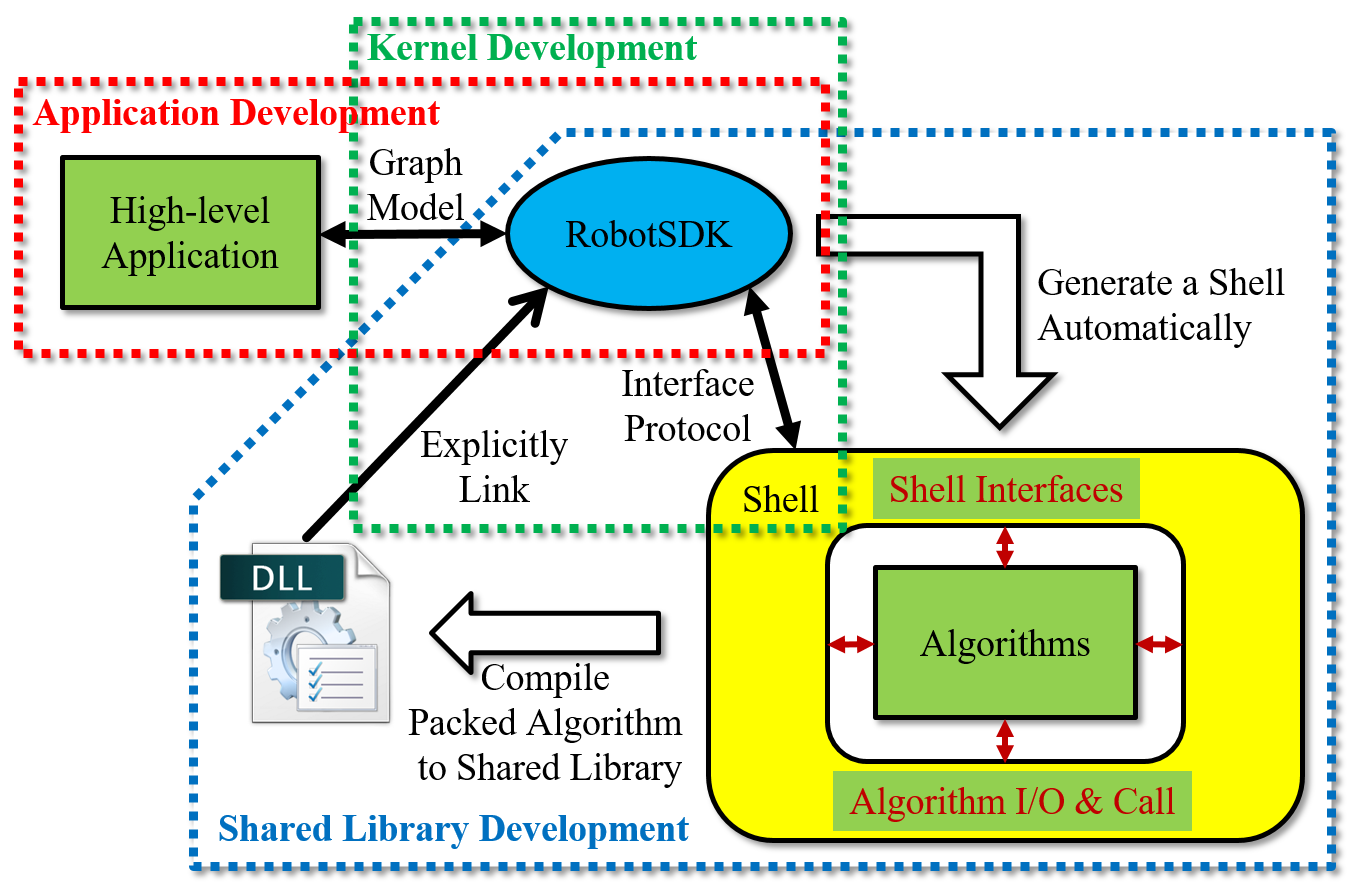
\includegraphics[width=0.9\textwidth]{./img/frame9}
		\end{center}
	\end{frame}
	
	\subsubsection{使用方法与实例(请通过网上视频与资料深入了解)}
	\begin{frame}{什么是RobotSDK---使用方法与实例}
		\begin{itemize}
			\item RobotSDK 4.0 的使用方法介绍视频:\url{https://youtu.be/uf7t8gWjN3U}
			\item RobotSDK 4.0 快速入门手册: \url{https://raw.githubusercontent.com/RobotSDK/RobotSDK/RobotSDK_4.0/RobotSDK4_QuickManual.pdf}
			\item RobotSDK 3.0 在北大Goblin小机器人上的使用(开发者方永\{方方土\}【kun显示不出来】):\url{https://youtu.be/ER-vk2F8UQU}
			\item RobotSDK 3.0 用于KITTI Dataset的处理和可视化:\url{https://youtu.be/Vgil3ObP3RE}
			\item RobotSDK 4.0 在筑波挑战赛(名古屋大学预赛)上使用:
			\begin{itemize}
				\item \url{https://youtu.be/syAKQ_JizRM}
				\item \url{https://youtu.be/yaWJ60fll_I}
			\end{itemize}
			\item RobotSDK 4.0 的第一个外部需求订单,DPM训练样本收集工具:\url{https://youtu.be/mjkYXEXnPMs}
			\item RobotSDK 4.0 在本人研究中的使用:\url{https://youtu.be/rAkuc5CNbl0}
		\end{itemize}
	\end{frame}
	
	\section{RobotSDK开源开发计划}
	\subsection{RobotSDK的发展简史}
	\subsubsection{北京大学时期}
	\begin{frame}{RobotSDK的发展简史---北京大学时期}
		\begin{block}{筑波挑战赛(2013.08-2013.09)}
			\begin{itemize}
				\item SensingPlatform SDK (RobotSDK 1.0)
				\begin{itemize}
					\item 尝试使用RobotSDK作为标准的软件开发工具(感谢陈向羽的耐心使用)。
					\item 只用于传感器数据的采集和可视化,算法编写没有采用RobotSDK。
				\end{itemize}
				\item 主要特点:
				\begin{itemize}
					\item 模块化软件设计基于\textcolor{red}{非抽象的底层图模型}。
					\item 模块化开发方式是\textcolor{red}{基于静态库的代码方式}。
					\item 无模板代码,接口需要自己写,同时RobotSDK内核代码需要嵌入工程,开发非常不便。
					\item 缺少数据池、数据流、数据缓冲和多线程的管理。					
				\end{itemize}
			\end{itemize}
		\end{block}
	\end{frame}
	\begin{frame}{RobotSDK的发展简史---北京大学时期}
		\begin{block}{筑波挑战赛之后(2013.09-2014.01)}
			\begin{itemize}
				\item SensorPlatform SDK (RobotSDK 2.0)
				\begin{itemize}
					\item 根据陈向羽的反馈和比赛中出的问题进行的一次重大升级。
					\item 部分实现了自顶向下的软件设计理念。
					\item 由代码方式转变为程序方式。
					\item 可以模块化算法代码。
				\end{itemize}
				\item 特点:
				\begin{itemize}
					\item 模块化软件设计基于\textcolor{red}{非抽象高层图模型}。
					\item 模块化开发方式\textcolor{red}{基于动态库的程序方式}。
					\item RobotSDK内核代码与工程实现了分离。
					\item 无模板代码,动态库开发不方便。
					\item 缺少数据池、数据流、数据缓冲和多线程的管理。	
					\item 部署方法非常麻烦。
				\end{itemize}
			\end{itemize}
		\end{block}
	\end{frame}
	\begin{frame}{RobotSDK的发展简史---北京大学时期}
		\begin{block}{离开北大前(2014.01-2014.08)}
			\begin{itemize}
				\item RobotSDK 2.1, 2.2, 3.0
				\begin{itemize}
					\item 完全实现了自顶向下的模块化软件开发理念。
					\item 开发了大量高层与底层辅助开发程序,用于高层与底层程序的开发。
					\item 较为成熟的RobotSDK 3.0以北京大学名义申请了软件著作权
					\item 并用于了本科生机器人课程教学。	
				\end{itemize}
				\item 特点:
				\begin{itemize}
					\item 模块化软件设计基于\textcolor{red}{抽象高层图模型}。
					\item 模块化开发方式引入了\textcolor{red}{预制代码模板},动态库开发与封装非常方便。
					\item 实现了基于抽象高层图模型的\textcolor{red}{抽象软件架构编程},高层程序具有\textcolor{red}{泛化能力}。
					\item 部分解决了数据池、数据流、数据缓冲和多线程的管理问题。
					\item 模块参数XML文件化,参数调整可以通过修改通用的XML文件实现。
					\item 节点类型仍然不够抽象(显式地分为“源”、“漏”、“中间节点”)。
				\end{itemize}
			\end{itemize}
		\end{block}
	\end{frame}
	
	\subsubsection{名古屋大学时期}
	\begin{frame}{RobotSDK的发展简史---名古屋大学时期}
		\begin{block}{名古屋大学时期(2014.09-2016.04)}
			\begin{itemize}
				\item RobotSDK 4.0
				\item 名古屋大学的研究需要RobotSDK能够处理高速多模块的情况,同时在使用ROS的过程中得到了一些启发。
				\item 在保留了RobotSDK 3.0的自顶向下模块化软件开发理念下,重写了内核,彻底解决了数据池、数据流、数据缓冲和多线程的管理问题。
				\item 实现了\textcolor{red}{高层程序的脚本化},并开发了\textcolor{red}{通用高层软件Robot-X},从而免去了编写高层程序的步骤。
				\item 多类节点被统一为一种通用节点(脚本化的前提)。
				\item \textcolor{red}{模块参数UI化}(基于C++11技术),参数直接可以通过Robot-X的通用参数修改器修改。
				\item 开发了一套完整的\textcolor{red}{RobotSDK Syntax}进一步简化了动态库的开发(基于C++11技术),使开发者只用关注于算法本身。
				\item 架设了\textcolor{red}{ROS接口},RobotSDK可以非常方便的与基于ROS的程序进行通信,同时本身也可以作为ROS的节点程序。
			\end{itemize}
		\end{block}
	\end{frame}
	
	\subsubsection{目前现状}
	\begin{frame}{RobotSDK的发展简史---目前现状}
		\begin{block}{好的方面}
			\begin{itemize}
				\item 经过了3年实践共6代升级,RobotSDK 4.0已经基本实现了一个稳定可靠的自顶向下模块化软件开发框架,最初的理念也已经实现。
				\item 北大方面,实验室的一些项目开始使用RobotSDK进行开发。
				\item 名大方面,他们开发的Autoware(基于ROS的无人车软件集)也集成了RobotSDK的部分功能。
				\item 我研究工作中的软件开发大部分基于RobotSDK实现。
			\end{itemize}
		\end{block}
		\begin{block}{不足的方面}
			\begin{itemize}
				\item 图模型的设计界面不够美观和强大,需要使用更专业的图模型库代替。
				\item RobotSDK基于队列的消息通信无法满足实时系统。
				\item 与ROS的融合度仍然不够。(ROS是一种程序间的模块化组织,RobotSDK是一种程序内的模块化组织,所以两者应该是互补的关系)
			\end{itemize}
		\end{block}
	\end{frame}
	
	\subsection{RobotSDK目前的开发计划}
	\begin{frame}{RobotSDK目前开发计划---卡耐基梅隆大学期间}
		\begin{enumerate}
			\item Java版的RobotSDK-JE(毕竟Java在CMU比较流行,但是实时系统就算了吧)
			\item RobotSDK-4.1: 
			\begin{itemize}
				\item 使用新的图模型库GOJS代替GraphViz;
				\item 使用ROS数据(Message)类型定义进行深度ROS融合;
				\item 开发独立的IDE平台Robot-Workshop,用于集成高层图模型设计(RobotSDK-4.0由Robot-X代劳)和底层模块编程工具(目前借由QtCreator平台进行编程)。
			\end{itemize}
			\item RobotSDK-4.2: 
			\begin{itemize}
				\item 基于高层抽象图模型的系统可行性认证与实时系统的时间规划(目前和UPenn在合作);
				\item 改进基于队列的通信为实时通信;
				\item 系统运行实时监控工具。
			\end{itemize}
		\end{enumerate}
	\end{frame}
	
	\subsection{RobotSDK开源开发计划}
	\begin{frame}{RobotSDK开源开发计划}
		\begin{itemize}
			\item RobotSDK目前只有我一个人负责开发和维护,而博士的工作越来越繁重,很多想法都没有时间实现。
			\item 同时本人也不是专业的软件工程出身,只是凭着个人兴趣和有限的能力在做这件事。
			\item 但是通过实践,个人认为这种自顶向下的模块化开发理念是有道理和优势的。
			\item 所以希望能有越来越多的人以RobotSDK为起始平台参与到这个项目的开发:
			\begin{itemize}
				\item 你可以来做内核开发和优化,以及目前最关键的是让它能够在实时系统下工作。
				\item 你可以来做辅助工具开发,让基于RobotSDK的开发更简单更有效率。
				\item 你可以来使用RobotSDK开发软件,同时分享自己的功能模块到社区,供别人参考使用。
			\end{itemize}
			\item RobotSDK的GitHub地址:\url{https://github.com/RobotSDK/RobotSDK}
			\item 谢谢大家!
		\end{itemize}
	\end{frame}
	
\end{document}
